\section{Experiments}
\label{sec:exp}

\subsection{Setup}
Image benchmarks are GQA, VizWiz, ScienceQA-IMG, TextVQA, POPE, MME, MMBench, MMMU, and AI2D~\cite{gqa,vizwiz,scienceqa,textvqa,pope,mme,mmbench,mmmu,ai2d}. Video benchmarks are MLVU, LongVideoBench, and Video-MME~\cite{mlvu,longvideobench,videomme}. POPE is F1. The six-task relative mean uses MME perception with denominator 1510.70, and GQA 61.90, POPE 85.80, MMBench 64.10, ScienceQA-IMG 69.51, and TextVQA 58.20. AI2D, MMMU, and VizWiz stay blank until their scores and denominators are recorded together. The main model is LLaVA-1.5-7B. Transfer tables reserve LLaVA-NeXT-7B, Qwen2.5-VL-7B, and LLaVA-OneVision-7B.

The seven comparison methods are SparseVLM and ViTCoP for salience and interaction, DivPrune and SCoRe for diversity and coverage, and AgilePruner, PruneSID, and CoIn for joint pre-decoder compression~\cite{agilepruner,prunesid}. Runs use NVIDIA V100 GPUs and lmms-eval at batch size one~\cite{lmmseval}. Layer-average capacity $\bar K=W/L$ aligns a flat entry with a layered schedule. On LLaVA-1.5-7B the three budgets are $\bar K\in\{128,64,32\}$, which remove 77.8\%, 88.9\%, and 94.4\% of the $576\times 32$ visual token-layer count. NeXT uses the same three ratios. Qwen2.5-VL-7B uses 80.2\% and 90.1\%. A dash means that cell has no measurement under this protocol. Published numbers from other papers are not copied into the table.

\subsection{LLaVA-1.5-7B}
\begin{table*}[t]
\centering
\scriptsize
\setlength{\tabcolsep}{2.6pt}
\caption{LLaVA-1.5-7B. Rel. is the mean of per-task scores divided by the fixed references. The filled row is the regional-quota basis plus QGE under the early schedule, and its Rel. uses the six measured tasks. MME is perception.}
\label{tab:main}
\begin{tabular*}{\textwidth}{@{\extracolsep{\fill}}l r r r r r r r r r r@{}}
\hline
Method & POPE & MME & MMB & MMMU & Text & AI2D & Viz & SQA & GQA & Rel. \\
\hline
\multicolumn{11}{l}{Dense reference, 576 visual tokens} \\
LLaVA-1.5-7B & 85.8 & 1510.7 & 64.1 & -- & 58.2 & -- & -- & 69.5 & 61.9 & 100.0\% \\
\hline
\multicolumn{11}{l}{Layer average $\bar K=128$ (77.8\% removed)} \\
SparseVLM~\cite{sparsevlm} & -- & -- & -- & -- & -- & -- & -- & -- & -- & -- \\
ViTCoP~\cite{vitcop} & -- & -- & -- & -- & -- & -- & -- & -- & -- & -- \\
DivPrune~\cite{divprune} & -- & -- & -- & -- & -- & -- & -- & -- & -- & -- \\
SCoRe~\cite{score} & -- & -- & -- & -- & -- & -- & -- & -- & -- & -- \\
AgilePruner~\cite{agilepruner} & -- & -- & -- & -- & -- & -- & -- & -- & -- & -- \\
PruneSID~\cite{prunesid} & -- & -- & -- & -- & -- & -- & -- & -- & -- & -- \\
CoIn~\cite{coin} & -- & -- & -- & -- & -- & -- & -- & -- & -- & -- \\
Q-SCOPE & -- & -- & -- & -- & -- & -- & -- & -- & -- & -- \\
\hline
\multicolumn{11}{l}{Layer average $\bar K=64$ (88.9\% removed)} \\
SparseVLM~\cite{sparsevlm} & -- & -- & -- & -- & -- & -- & -- & -- & -- & -- \\
ViTCoP~\cite{vitcop} & -- & -- & -- & -- & -- & -- & -- & -- & -- & -- \\
DivPrune~\cite{divprune} & -- & -- & -- & -- & -- & -- & -- & -- & -- & -- \\
SCoRe~\cite{score} & -- & -- & -- & -- & -- & -- & -- & -- & -- & -- \\
AgilePruner~\cite{agilepruner} & -- & -- & -- & -- & -- & -- & -- & -- & -- & -- \\
PruneSID~\cite{prunesid} & -- & -- & -- & -- & -- & -- & -- & -- & -- & -- \\
CoIn~\cite{coin} & -- & -- & -- & -- & -- & -- & -- & -- & -- & -- \\
Q-SCOPE & -- & -- & -- & -- & -- & -- & -- & -- & -- & -- \\
\hline
\multicolumn{11}{l}{Layer average $\bar K=32$ (94.4\% removed)} \\
SparseVLM~\cite{sparsevlm} & -- & -- & -- & -- & -- & -- & -- & -- & -- & -- \\
ViTCoP~\cite{vitcop} & -- & -- & -- & -- & -- & -- & -- & -- & -- & -- \\
DivPrune~\cite{divprune} & -- & -- & -- & -- & -- & -- & -- & -- & -- & -- \\
SCoRe~\cite{score} & -- & -- & -- & -- & -- & -- & -- & -- & -- & -- \\
AgilePruner~\cite{agilepruner} & -- & -- & -- & -- & -- & -- & -- & -- & -- & -- \\
PruneSID~\cite{prunesid} & -- & -- & -- & -- & -- & -- & -- & -- & -- & -- \\
CoIn~\cite{coin} & -- & -- & -- & -- & -- & -- & -- & -- & -- & -- \\
Q-SCOPE & 86.2 & 1409.0 & 61.6 & -- & 53.3 & -- & -- & 69.9 & 57.1 & 95.66\% \\
\hline
\end{tabular*}
\end{table*}

At the 94.4\% budget, regional quotas plus QGE score POPE 86.2, MME perception 1409.0, MMBench 61.6, TextVQA 53.3, ScienceQA-IMG 69.9, and GQA 57.1. ScienceQA-IMG and POPE stay near the unpruned references. GQA and TextVQA remain lower. The other two budgets and every external method are blank.

\subsection{Transfer and video}
Tables~\ref{tab:next} and~\ref{tab:qwen} use the six classic tasks. Each model is normalized by its own unpruned scores. Qwen is split into 80.2\% and 90.1\% removal. Both tables are unfilled. Video uses LLaVA-OneVision-7B on MLVU, LongVideoBench, and Video-MME at two retained lengths. Those cells are unfilled as well.

\begin{table}[t]
\centering
\scriptsize
\setlength{\tabcolsep}{2pt}
\caption{LLaVA-NeXT-7B. Six tasks. Scores are unfilled.}
\label{tab:next}
\begin{tabular}{@{}lrrrrrr r@{}}
\hline
Method & MME & MMB & POPE & SQA & GQA & Text & Rel. \\
\hline
Dense & -- & -- & -- & -- & -- & -- & 100\% \\
\multicolumn{8}{@{}l}{77.8\% / 88.9\% / 94.4\% removed} \\
ViTCoP & -- & -- & -- & -- & -- & -- & -- \\
SCoRe & -- & -- & -- & -- & -- & -- & -- \\
CoIn & -- & -- & -- & -- & -- & -- & -- \\
Q-SCOPE & -- & -- & -- & -- & -- & -- & -- \\
\hline
\end{tabular}
\end{table}

\begin{table}[t]
\centering
\scriptsize
\setlength{\tabcolsep}{2pt}
\caption{Qwen2.5-VL-7B at 80.2\% and 90.1\% removal. Scores are unfilled.}
\label{tab:qwen}
\begin{tabular}{@{}lrrrrrr r@{}}
\hline
Method & MME & MMB & POPE & SQA & GQA & Text & Rel. \\
\hline
Dense & -- & -- & -- & -- & -- & -- & 100\% \\
\multicolumn{8}{@{}l}{80.2\% removed} \\
ViTCoP & -- & -- & -- & -- & -- & -- & -- \\
SCoRe & -- & -- & -- & -- & -- & -- & -- \\
CoIn & -- & -- & -- & -- & -- & -- & -- \\
Q-SCOPE & -- & -- & -- & -- & -- & -- & -- \\
\multicolumn{8}{@{}l}{90.1\% removed} \\
ViTCoP & -- & -- & -- & -- & -- & -- & -- \\
SCoRe & -- & -- & -- & -- & -- & -- & -- \\
CoIn & -- & -- & -- & -- & -- & -- & -- \\
Q-SCOPE & -- & -- & -- & -- & -- & -- & -- \\
\hline
\end{tabular}
\end{table}

\begin{table}[t]
\centering
\scriptsize
\setlength{\tabcolsep}{3pt}
\caption{Video. MLVU, LongVideoBench, and Video-MME are unfilled.}
\label{tab:video}
\begin{tabular}{@{}lrrr@{}}
\hline
Method & MLVU & LVB & V-MME \\
\hline
Dense & -- & -- & -- \\
ViTCoP & -- & -- & -- \\
DivPrune & -- & -- & -- \\
SCoRe & -- & -- & -- \\
CoIn & -- & -- & -- \\
Q-SCOPE & -- & -- & -- \\
\hline
\end{tabular}
\end{table}

\subsection{Efficiency}
Efficiency has not been measured. The planned comparison, on one V100 with the same images and batch size 1, is the unpruned model, ViTCoP, SCoRe, CoIn, Q-SCOPE without QGE, and full Q-SCOPE. Accuracy runs stop naturally. Timing uses a fixed generation length so answer length does not enter the clock. Time to first token starts from the image and text already in memory and includes the vision tower, projection, basis, QGE, and prefill. The same run records generation time, peak memory, and the selector time. Warmup is excluded. Each setting is repeated, and we report the median, mean, and tail. Equal $W$ only matches the visual token-layer count.

\subsection{Ablations}
With QGE off and MME as the perception-plus-cognition total, middle features lead GQA and POPE, deep features lead MMBench, and dual-depth plus the older coverage leads the four-task relative mean (Table~\ref{tab:depth}). This protocol uses $W{=}2048$ and is not the 94.4\% row above. On 1,024 images the mean Jaccard of the middle and deep top sets is 0.331. On MMBench, 35 questions are correct for the middle depth and for dual-depth but wrong for the deep depth, and 38 show the opposite pattern. Dual-depth supplies two rankings. It does not win every task.

\begin{table}[t]
\centering
\scriptsize
\setlength{\tabcolsep}{3pt}
\caption{Dual-depth, QGE off. MME-T is the total score. Rel.4 uses these four tasks only.}
\label{tab:depth}
\begin{tabular}{@{}lrrrrr@{}}
\hline
Guide & GQA & POPE & MME-T & MMB & Rel.4 \\
\hline
Middle & 57.9 & 84.0 & 1718.0 & 62.0 & 95.2 \\
Deep & 56.4 & 81.3 & 1745.7 & 63.0 & 94.6 \\
Dual-depth & 57.4 & 82.8 & 1744.5 & 62.6 & 95.3 \\
Dual-depth + cover & 57.2 & 83.0 & 1765.2 & 62.2 & 95.4 \\
\hline
\end{tabular}
\end{table}

\begin{table}[t]
\centering
\scriptsize
\setlength{\tabcolsep}{2.4pt}
\caption{Coverage variants, QGE off. MME is perception.}
\label{tab:cover}
\begin{tabular}{@{}lrrrr@{}}
\hline
Rule & POPE & MME & Text & Rel.6 \\
\hline
Previous cover & 81.5 & 1339.3 & 53.5 & 93.5 \\
Valid prototypes & 81.5 & 1349.5 & 53.5 & 93.5 \\
Drop empty-cell salience & 76.4 & 1299.0 & 53.0 & 91.0 \\
Update prototypes & 82.2 & 1372.0 & 53.8 & 93.8 \\
Regional quota & 81.5 & 1376.4 & 53.9 & 93.9 \\
Wider residual pool & 81.1 & 1363.8 & 53.9 & 93.3 \\
\hline
\end{tabular}
\end{table}

Regional quotas are the strongest of these coverage variants, at 93.89\% on the six-task mean in the unrounded record. Removing salience on empty cells drops POPE to 76.33. On that quota basis, the smallest QGE budget raises the six-task mean from 93.89\% to 95.66\%. GQA moves from 55.92 to 57.08, with 498 newly correct answers and 353 newly incorrect ones. POPE rises and TextVQA falls, from 53.85 to 53.28. Larger exchange budgets keep lifting POPE and lower the other tasks together. The same $W{=}1024$ with a late first cut scores 93.47\%, against 87.67\% and 87.45\% for two earlier cuts. The late schedule has the smaller entry and the higher score. Changing only the last stage moves the six-task mean by 0.11 points, from 96.78\% to 96.89\%.

\begin{figure}[t]
\centering
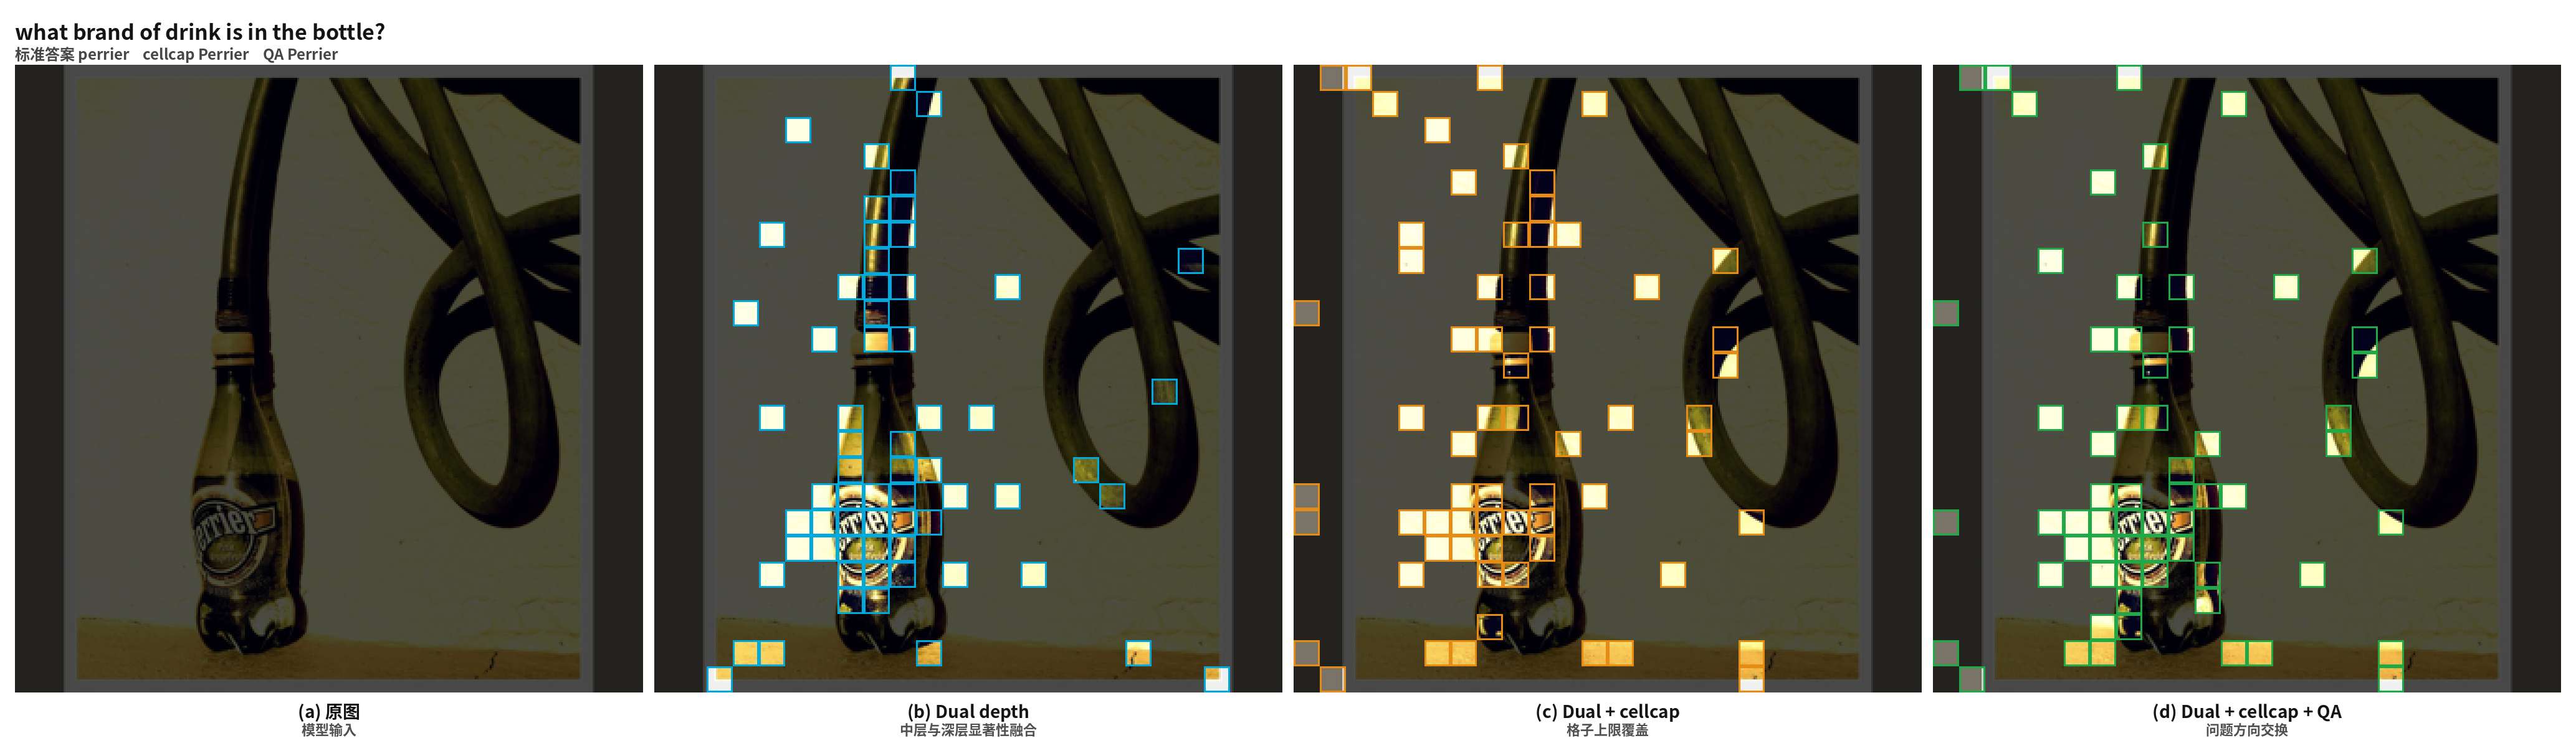
\includegraphics[width=\linewidth]{figures/textvqa_bottle.png}
\caption{TextVQA bottle. Dim cells are dropped. From left to right: input, dual-depth, regional quota, and QGE. Both the quota basis and QGE answer Perrier.}
\label{fig:bottle}
\end{figure}

\begin{figure}[t]
\centering
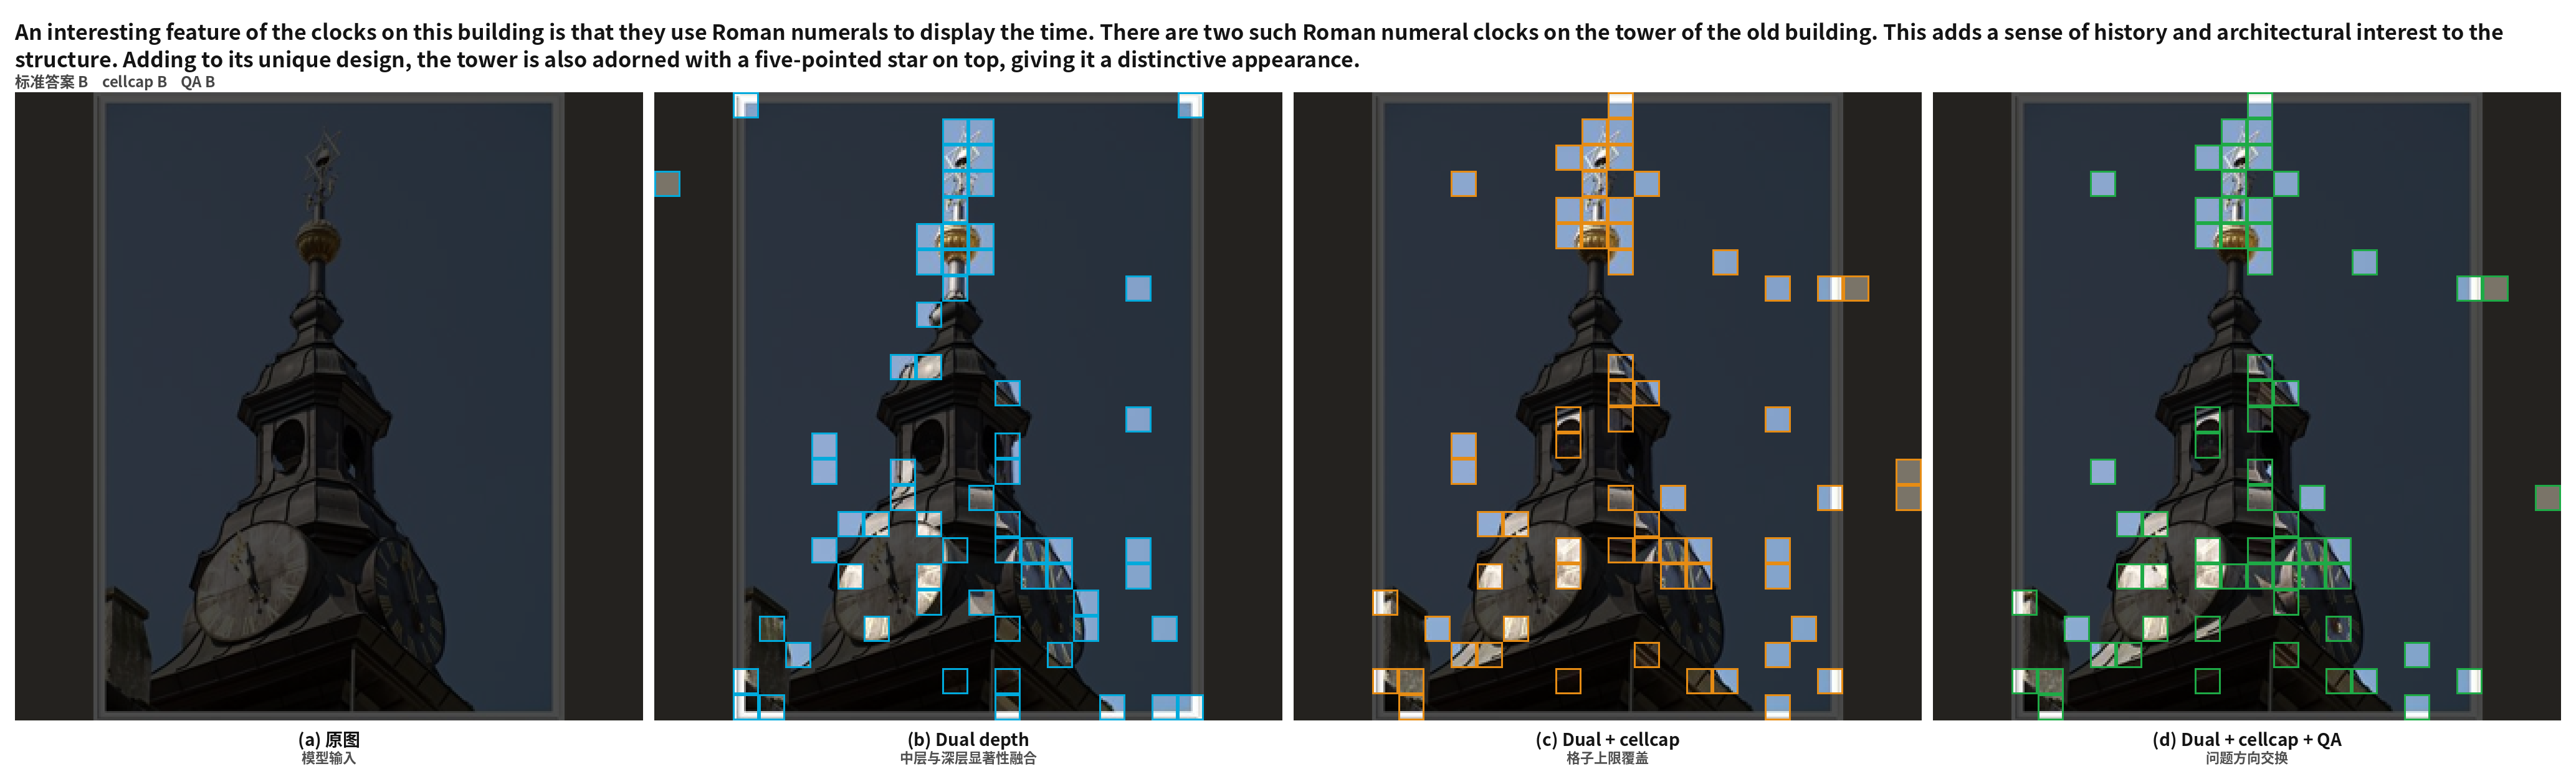
\includegraphics[width=\linewidth]{figures/mmbench_clock.png}
\caption{MMBench clock. The quota adds peripheral cells. QGE moves part of the selection back onto the clock face. Both answer B.}
\label{fig:clock}
\end{figure}
